\chapter{The Unknown}

Day, for which Dantès had so eagerly and impatiently waited with open
eyes, again dawned. With the first light Dantès resumed his search.
Again he climbed the rocky height he had ascended the previous evening,
and strained his view to catch every peculiarity of the landscape; but
it wore the same wild, barren aspect when seen by the rays of the
morning sun which it had done when surveyed by the fading glimmer of
eve.

Descending into the grotto, he lifted the stone, filled his pockets
with gems, put the box together as well and securely as he could,
sprinkled fresh sand over the spot from which it had been taken, and
then carefully trod down the earth to give it everywhere a uniform
appearance; then, quitting the grotto, he replaced the stone, heaping
on it broken masses of rocks and rough fragments of crumbling granite,
filling the interstices with earth, into which he deftly inserted
rapidly growing plants, such as the wild myrtle and flowering thorn,
then carefully watering these new plantations, he scrupulously effaced
every trace of footsteps, leaving the approach to the cavern as
savage-looking and untrodden as he had found it. This done, he
impatiently awaited the return of his companions. To wait at Monte
Cristo for the purpose of watching like a dragon over the almost
incalculable riches that had thus fallen into his possession satisfied
not the cravings of his heart, which yearned to return to dwell among
mankind, and to assume the rank, power, and influence which are always
accorded to wealth—that first and greatest of all the forces within the
grasp of man.

On the sixth day, the smugglers returned. From a distance Dantès
recognized the rig and handling of \textit{La Jeune Amélie}, and dragging
himself with affected difficulty towards the landing-place, he met his
companions with an assurance that, although considerably better than
when they quitted him, he still suffered acutely from his late
accident. He then inquired how they had fared in their trip. To this
question the smugglers replied that, although successful in landing
their cargo in safety, they had scarcely done so when they received
intelligence that a guard-ship had just quitted the port of Toulon and
was crowding all sail towards them. This obliged them to make all the
speed they could to evade the enemy, when they could but lament the
absence of Dantès, whose superior skill in the management of a vessel
would have availed them so materially. In fact, the pursuing vessel had
almost overtaken them when, fortunately, night came on, and enabled
them to double the Cape of Corsica, and so elude all further pursuit.
Upon the whole, however, the trip had been sufficiently successful to
satisfy all concerned; while the crew, and particularly Jacopo,
expressed great regrets that Dantès had not been an equal sharer with
themselves in the profits, which amounted to no less a sum than fifty
piastres each.

\begin{figure}[ht]
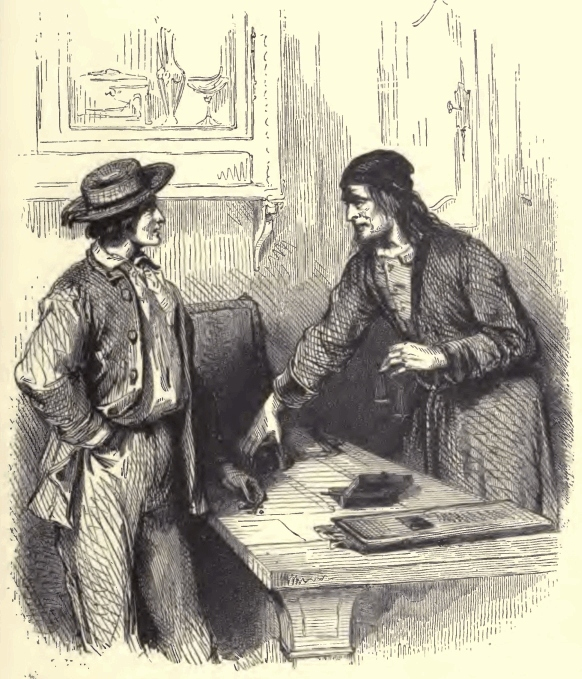
\includegraphics[width=\textwidth]{0311m.jpg}
\end{figure}

Edmond preserved the most admirable self-command, not suffering the
faintest indication of a smile to escape him at the enumeration of all
the benefits he would have reaped had he been able to quit the island;
but as \textit{La Jeune Amélie} had merely come to Monte Cristo to fetch him
away, he embarked that same evening, and proceeded with the captain to
Leghorn.

Arrived at Leghorn, he repaired to the house of a Jew, a dealer in
precious stones, to whom he disposed of four of his smallest diamonds
for five thousand francs each. Dantès half feared that such valuable
jewels in the hands of a poor sailor like himself might excite
suspicion; but the cunning purchaser asked no troublesome questions
concerning a bargain by which he gained a round profit of at least
eighty per cent.

The following day Dantès presented Jacopo with an entirely new vessel,
accompanying the gift by a donation of one hundred piastres, that he
might provide himself with a suitable crew and other requisites for his
outfit, upon condition that he would go at once to Marseilles for the
purpose of inquiring after an old man named Louis Dantès, residing in
the Allées de Meilhan, and also a young woman called Mercédès, an
inhabitant of the Catalan village.

Jacopo could scarcely believe his senses at receiving this magnificent
present, which Dantès hastened to account for by saying that he had
merely been a sailor from whim and a desire to spite his family, who
did not allow him as much money as he liked to spend; but that on his
arrival at Leghorn he had come into possession of a large fortune, left
him by an uncle, whose sole heir he was. The superior education of
Dantès gave an air of such extreme probability to this statement that
it never once occurred to Jacopo to doubt its accuracy.

The term for which Edmond had engaged to serve on board \textit{La Jeune
Amélie} having expired, Dantès took leave of the captain, who at first
tried all his powers of persuasion to induce him to remain as one of
the crew, but having been told the history of the legacy, he ceased to
importune him further.

The following morning Jacopo set sail for Marseilles, with directions
from Dantès to join him at the Island of Monte Cristo.

Having seen Jacopo fairly out of the harbor, Dantès proceeded to make
his final adieus on board \textit{La Jeune Amélie}, distributing so liberal a
gratuity among her crew as to secure for him the good wishes of all,
and expressions of cordial interest in all that concerned him. To the
captain he promised to write when he had made up his mind as to his
future plans. Then Dantès departed for Genoa.

At the moment of his arrival a small yacht was under trial in the bay;
this yacht had been built by order of an Englishman, who, having heard
that the Genoese excelled all other builders along the shores of the
Mediterranean in the construction of fast-sailing vessels, was desirous
of possessing a specimen of their skill; the price agreed upon between
the Englishman and the Genoese builder was forty thousand francs.
Dantès, struck with the beauty and capability of the little vessel,
applied to its owner to transfer it to him, offering sixty thousand
francs, upon condition that he should be allowed to take immediate
possession. The proposal was too advantageous to be refused, the more
so as the person for whom the yacht was intended had gone upon a tour
through Switzerland, and was not expected back in less than three weeks
or a month, by which time the builder reckoned upon being able to
complete another. A bargain was therefore struck. Dantès led the owner
of the yacht to the dwelling of a Jew; retired with the latter for a
few minutes to a small back parlor, and upon their return the Jew
counted out to the shipbuilder the sum of sixty thousand francs in
bright gold pieces.

The delighted builder then offered his services in providing a suitable
crew for the little vessel, but this Dantès declined with many thanks,
saying he was accustomed to cruise about quite alone, and his principal
pleasure consisted in managing his yacht himself; the only thing the
builder could oblige him in would be to contrive a sort of secret
closet in the cabin at his bed’s head, the closet to contain three
divisions, so constructed as to be concealed from all but himself. The
builder cheerfully undertook the commission, and promised to have these
secret places completed by the next day, Dantès furnishing the
dimensions and plan in accordance with which they were to be
constructed.

\begin{figure}[ht]
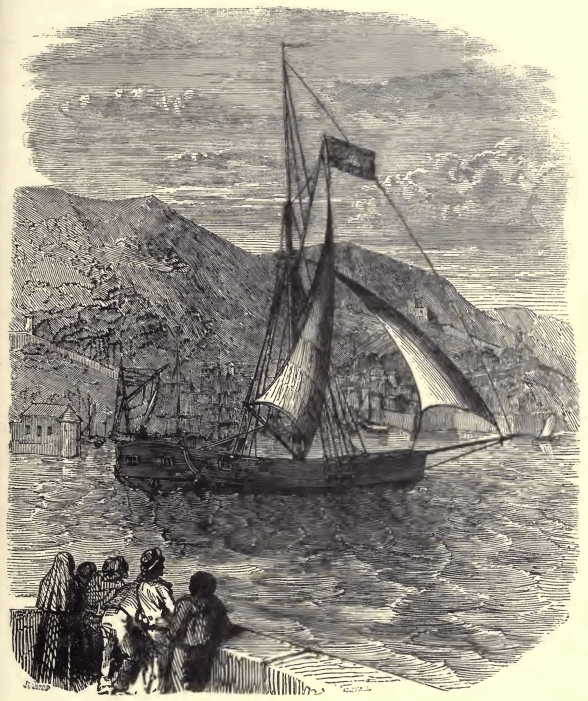
\includegraphics[width=\textwidth]{0313m.jpg}
\end{figure}

Two hours afterward Dantès sailed from the port of Genoa, under the
inspection of an immense crowd drawn together by curiosity to see the
rich Spanish nobleman who preferred managing his own yacht. But their
wonder was soon changed to admiration at seeing the perfect skill with
which Dantès handled the helm. The boat, indeed, seemed to be animated
with almost human intelligence, so promptly did it obey the slightest
touch; and Dantès required but a short trial of his beautiful craft to
acknowledge that the Genoese had not without reason attained their high
reputation in the art of shipbuilding.

The spectators followed the little vessel with their eyes as long as it
remained visible; they then turned their conjectures upon her probable
destination. Some insisted she was making for Corsica, others the
Island of Elba; bets were offered to any amount that she was bound for
Spain; while Africa was positively reported by many persons as her
intended course; but no one thought of Monte Cristo.

Yet thither it was that Dantès guided his vessel, and at Monte Cristo
he arrived at the close of the second day; his boat had proved herself
a first-class sailor, and had come the distance from Genoa in
thirty-five hours. Dantès had carefully noted the general appearance of
the shore, and, instead of landing at the usual place, he dropped
anchor in the little creek. The island was utterly deserted, and bore
no evidence of having been visited since he went away; his treasure was
just as he had left it.

Early on the following morning he commenced the removal of his riches,
and ere nightfall the whole of his immense wealth was safely deposited
in the compartments of the secret locker.

A week passed by. Dantès employed it in manœuvring his yacht round the
island, studying it as a skilful horseman would the animal he destined
for some important service, till at the end of that time he was
perfectly conversant with its good and bad qualities. The former Dantès
proposed to augment, the latter to remedy.

Upon the eighth day he discerned a small vessel under full sail
approaching Monte Cristo. As it drew near, he recognized it as the boat
he had given to Jacopo. He immediately signalled it. His signal was
returned, and in two hours afterwards the new-comer lay at anchor
beside the yacht.

A mournful answer awaited each of Edmond’s eager inquiries as to the
information Jacopo had obtained. Old Dantès was dead, and Mercédès had
disappeared.

Dantès listened to these melancholy tidings with outward calmness; but,
leaping lightly ashore, he signified his desire to be quite alone. In a
couple of hours he returned. Two of the men from Jacopo’s boat came on
board the yacht to assist in navigating it, and he gave orders that she
should be steered direct to Marseilles. For his father’s death he was
in some manner prepared; but he knew not how to account for the
mysterious disappearance of Mercédès.

Without divulging his secret, Dantès could not give sufficiently clear
instructions to an agent. There were, besides, other particulars he was
desirous of ascertaining, and those were of a nature he alone could
investigate in a manner satisfactory to himself. His looking-glass had
assured him, during his stay at Leghorn, that he ran no risk of
recognition; moreover, he had now the means of adopting any disguise he
thought proper. One fine morning, then, his yacht, followed by the
little fishing-boat, boldly entered the port of Marseilles, and
anchored exactly opposite the spot from whence, on the
never-to-be-forgotten night of his departure for the Château d’If, he
had been put on board the boat destined to convey him thither.

\begin{figure}[ht]
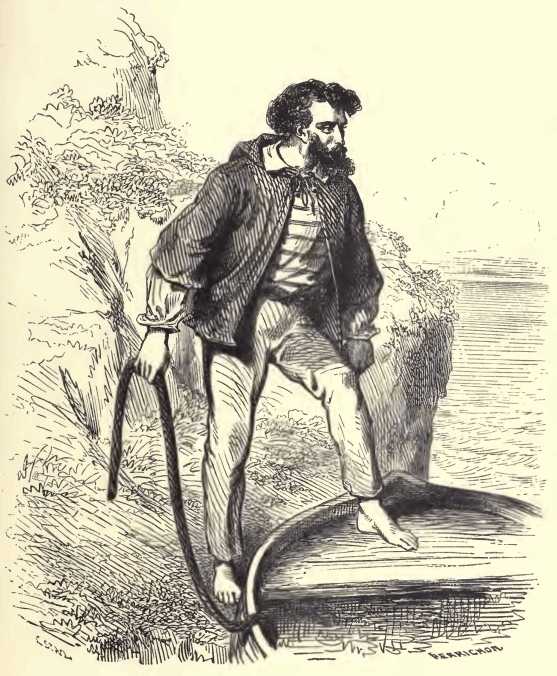
\includegraphics[width=\textwidth]{0315m.jpg}
\end{figure}

Still Dantès could not view without a shudder the approach of a
gendarme who accompanied the officers deputed to demand his bill of
health ere the yacht was permitted to hold communication with the
shore; but with that perfect self-possession he had acquired during his
acquaintance with Faria, Dantès coolly presented an English passport he
had obtained from Leghorn, and as this gave him a standing which a
French passport would not have afforded, he was informed that there
existed no obstacle to his immediate debarkation.

The first person to attract the attention of Dantès, as he landed on
the Canebière, was one of the crew belonging to the \textit{Pharaon}. Edmond
welcomed the meeting with this fellow—who had been one of his own
sailors—as a sure means of testing the extent of the change which time
had worked in his own appearance. Going straight towards him, he
propounded a variety of questions on different subjects, carefully
watching the man’s countenance as he did so; but not a word or look
implied that he had the slightest idea of ever having seen before the
person with whom he was then conversing.

Giving the sailor a piece of money in return for his civility, Dantès
proceeded onwards; but ere he had gone many steps he heard the man
loudly calling him to stop.

Dantès instantly turned to meet him.

“I beg your pardon, sir,” said the honest fellow, in almost breathless
haste, “but I believe you made a mistake; you intended to give me a
two-franc piece, and see, you gave me a double Napoleon.”

“Thank you, my good friend. I see that I have made a trifling mistake,
as you say; but by way of rewarding your honesty I give you another
double Napoleon, that you may drink to my health, and be able to ask
your messmates to join you.”

So extreme was the surprise of the sailor, that he was unable even to
thank Edmond, whose receding figure he continued to gaze after in
speechless astonishment. “Some nabob from India,” was his comment.

Dantès, meanwhile, went on his way. Each step he trod oppressed his
heart with fresh emotion; his first and most indelible recollections
were there; not a tree, not a street, that he passed but seemed filled
with dear and cherished memories. And thus he proceeded onwards till he
arrived at the end of the Rue de Noailles, from whence a full view of
the Allées de Meilhan was obtained. At this spot, so pregnant with fond
and filial remembrances, his heart beat almost to bursting, his knees
tottered under him, a mist floated over his sight, and had he not clung
for support to one of the trees, he would inevitably have fallen to the
ground and been crushed beneath the many vehicles continually passing
there. Recovering himself, however, he wiped the perspiration from his
brows, and stopped not again till he found himself at the door of the
house in which his father had lived.

The nasturtiums and other plants, which his father had delighted to
train before his window, had all disappeared from the upper part of the
house.

Leaning against the tree, he gazed thoughtfully for a time at the upper
stories of the shabby little house. Then he advanced to the door, and
asked whether there were any rooms to be let. Though answered in the
negative, he begged so earnestly to be permitted to visit those on the
fifth floor, that, in despite of the oft-repeated assurance of the
\textit{concierge} that they were occupied, Dantès succeeded in inducing the
man to go up to the tenants, and ask permission for a gentleman to be
allowed to look at them.

The tenants of the humble lodging were a young couple who had been
scarcely married a week; and seeing them, Dantès sighed heavily.
Nothing in the two small chambers forming the apartments remained as it
had been in the time of the elder Dantès; the very paper was different,
while the articles of antiquated furniture with which the rooms had
been filled in Edmond’s time had all disappeared; the four walls alone
remained as he had left them.

The bed belonging to the present occupants was placed as the former
owner of the chamber had been accustomed to have his; and, in spite of
his efforts to prevent it, the eyes of Edmond were suffused in tears as
he reflected that on that spot the old man had breathed his last,
vainly calling for his son.

The young couple gazed with astonishment at the sight of their
visitor’s emotion, and wondered to see the large tears silently chasing
each other down his otherwise stern and immovable features; but they
felt the sacredness of his grief, and kindly refrained from questioning
him as to its cause, while, with instinctive delicacy, they left him to
indulge his sorrow alone.

\begin{figure}[h]
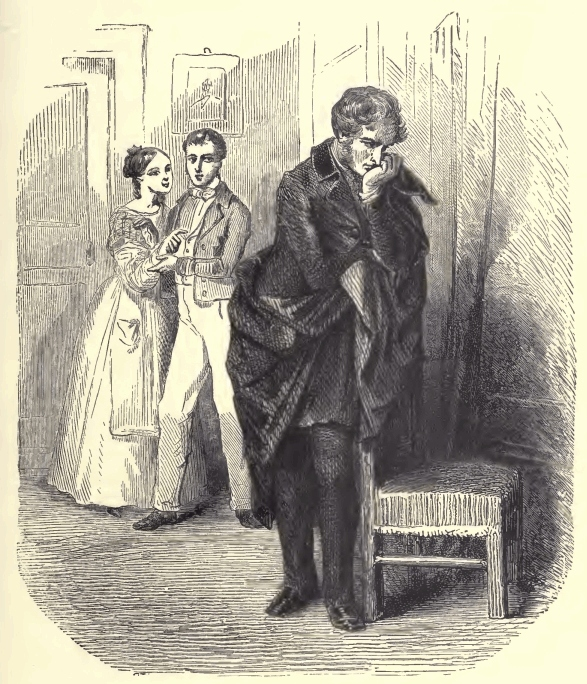
\includegraphics[width=\textwidth]{0317m.jpg}
\end{figure}

When he withdrew from the scene of his painful recollections, they both
accompanied him downstairs, reiterating their hope that he would come
again whenever he pleased, and assuring him that their poor dwelling
would ever be open to him.

As Edmond passed the door on the fourth floor, he paused to inquire
whether Caderousse the tailor still dwelt there; but he received for
reply, that the person in question had got into difficulties, and at
the present time kept a small inn on the route from Bellegarde to
Beaucaire.

Having obtained the address of the person to whom the house in the
Allées de Meilhan belonged, Dantès next proceeded thither, and, under
the name of Lord Wilmore (the name and title inscribed on his
passport), purchased the small dwelling for the sum of twenty-five
thousand francs, at least ten thousand more than it was worth; but had
its owner asked half a million, it would unhesitatingly have been
given.

The very same day the occupants of the apartments on the fifth floor of
the house, now become the property of Dantès, were duly informed by the
notary who had arranged the necessary transfer of deeds, etc., that the
new landlord gave them their choice of any of the rooms in the house,
without the least augmentation of rent, upon condition of their giving
instant possession of the two small chambers they at present inhabited.

This strange event aroused great wonder and curiosity in the
neighborhood of the Allées de Meilhan, and a multitude of theories were
afloat, none of which was anywhere near the truth. But what raised
public astonishment to a climax, and set all conjecture at defiance,
was the knowledge that the same stranger who had in the morning visited
the Allées de Meilhan had been seen in the evening walking in the
little village of the Catalans, and afterwards observed to enter a poor
fisherman’s hut, and to pass more than an hour in inquiring after
persons who had either been dead or gone away for more than fifteen or
sixteen years.

But on the following day the family from whom all these particulars had
been asked received a handsome present, consisting of an entirely new
fishing-boat, with two seines and a tender.

The delighted recipients of these munificent gifts would gladly have
poured out their thanks to their generous benefactor, but they had seen
him, upon quitting the hut, merely give some orders to a sailor, and
then springing lightly on horseback, leave Marseilles by the Porte
d’Aix.
